
\documentclass[12pt]{article}

\usepackage{mphysproject}
\usepackage[T1]{fontenc} 

\usepackage{hyperref}  

\usepackage[style=numeric, sorting=none]{biblatex}
\usepackage{amssymb}
\addbibresource{references.bib}
\usepackage{color, soul}

\usepackage{tikz}
\usepackage{subfig}
\usetikzlibrary{knots}

\begin{document}

\title{Machine Learning for Knot Discovery} % Place your project title in here
\author{D. P. Mihajlovic} % Put your name here
\supervisor{Professor D. Michieletto} % Place your principal supervisor here
%\supervisor{Dr A. Smith} % If you have additional supervisors, list them with separate \supervisor commands
\date{} % Today's date will appear on the title page by default, but if you want to tie this to a particular date, you can do so here

% Insert your abstract below
\begin{abstract}
The abstract is a concise outline of the project, summarising (i) the research question addressed by the project; (ii) the motivation for that research question; (iii) the main method you used to answer it; (iv) your main result; and (v) the implications of this result in the field of study. Aim for one sentence (on average) for each. The entire abstract should be no more than 100 words, and should not contain display equations or references.
\end{abstract}

% This command is essential to make the title page appear: DO NOT REMOVE IT
\maketitle

% This command introduces the Personal Statement: DO NOT REMOVE IT
\personalstatement

\begin{it}

Insert a personal statement of around one page (maximum two) that sets out the nature of the various tasks conducted in the project and an indication of the amount of time spent on them. You should highlight any unanticipated difficulties you encountered in the project, as this may help the assessors better understand---for example---why the quality or quantity of data obtained is less than one might normally expect. This statement may also help assessors understand your individual contribution to the work described in the report: however, this should also be evident from the report itself.

The example below was submitted by a former MPhys Project student.

\end{it}

% I spent the first 6 weeks meeting regularly with my supervisor and becoming familiar with the equipment I would be using. I needed to learn about the electronic workings of the experimental system and the programming control I would be administering. I found this initially very time consuming but achieved it by working through the manuals for the pieces of equipment I would be using. I also ran and edited C++ code from an existing package I was given by my supervisor. I was fairly unfamiliar with C++ and so running existing code was a good way for me to begin to understand the language and also the way it could be used to control the equipment.

% Outside the lab I began reading articles, LHCb manuals and information from the LHCb website that explained the workings of Multi-Anode Photomultiplier Tubes and how they were being incorporated into the LHCb experiment. As work in the lab was very much about coding and electronics at this stage it was easy to lose sight of the overall goal and so researching such topics kept me focused.

% There was a problem with the QDC (charge to digital converter) module I was using, but after switching to the other one I was able to progress. I spent the next 5 weeks administering signals to the QDC module with an external pulse generator. This way I could view the pulse with an oscilloscope and manually set the characteristics I wished to use (width, period etc) before interpreting the resulting data. I edited the C++ code in order to produce text files containing information about each pulse of light, or `event', being administered. This information was in the form of ADC counts (digital conversions of analogue signals).

% During this time, and continuing on through the Christmas break, I continued to research MaPMTs. I conducted a literature review and used this to compile the background knowledge section of my report. The LHCb manuals I was given by supervisor proved to be very informative and provided much of the information for this section. I not only focused on MaPMTs but looked into the Hybrid Photon Detector (HPD) models which are currently used in the LHCb experiment and that the MaPMTs are due to replace.

% In Semester 2 I was able to use the MaPMT to obtain data. After initially being introduced to the MaPMT by my supervisor, I spent the first week familiarising myself with how it worked. My supervisor helped me set up an LED pulse which was directed to the photocathode surface of the MaPMT. I spent the next 3 weeks adjusting the equipment to cope with the new pulse source and taking data runs. Much of the code I had worked on in Semester 1 was useful here with constant improvements being made throughout the course of the semester.

% I spent the next 2 weeks working learning about the graphical tool ROOT and using it to produce histograms of my results. I was continued working on my report with the Experimental Method section coming to form.

% The following 2 weeks were spent altering experimental parameters such as the voltage being administered to the MaPMT and producing further histograms. I spent the remainder of my time analysing my histograms and working on my report.

% If you have anyone that needs to be acknowledged (e.g., anyone who provided assistance with your project work,
% provided data etc) please do so here. Delete this (or comment it out) if you have no-one to acknowledge.
\acknowledgments

\begin{it}
If you received any assistance with your project (beyond the usual advice and support from your supervisor), this should be recorded in a section headed Acknowledgements at the end of your Personal Statement. You should also note here if your MPhys Project follows on from an earlier project (e.g., Senior Honours or a summer project) so that assessors can focus on the new work conducted during the MPhys project study period.

Speak to your supervisor or the course organiser if you are not sure about what might be relevant to include here.
\end{it}

Much of the good advice to students for conducting the MPhys Project and writing the report was created by the previous Course Organiser, Victoria Martin. I have tried to incorporate as much as this as possible into the current generation of course materials. Any bugs in the \LaTeX\ style file are entirely my own.


% This command inserts a table of contents, and sets things up for the main text of your report.
% The page count starts from here. DO NOT DELETE OR DISABLE THIS COMMAND!
\maintext

\section{Introduction}

% \begin{it}
% The key point to reach by the end of the introduction is a clear statement of what the specific research question that you investigated in the project, and what it was the motivated this question. Typically this is done by first setting the scene with a description of the general subject area as a whole.  Then you would highlight key scientific developments that make the question you have investigated (i) relevant and (ii) lacking an answer.

% It is common for introductions to end with a brief sketch of the main content of the rest of the report; there is no harm in summarising the conclusion, as this can help the reader pace themselves as they work through your report.
% \end{it}

\hl{Intro to knot theory/ applications in physics/ need for knot invariant and classification -> lead onto the general idea of a classification problem : ML is known to be well suited to this}

Knot theory is the study of knots: self-entangled, closed loops in $\mathbb{R}^{3}$. It doesn't take too much searching to discover the ubiquity of these such knots, stretching from the super-coiling nature of DNA \cite{bauer1980supercoiled} to forms of the path integral in a topological quantum field theory \cite{witten1994quantum}. The abundance of knots in such physical systems highlights the importance of knot theory and its study in physics.

The search for a unique, invariant property of knots has eluded mathematicians and physicists since the foundations of knot theory in the $19^{th}$ century. In searching for such a property, academics have unveiled a plethora of methods that categorize and distinguish knots to increasing levels of complexity (i.e.\ number of crossings) - however, each of these methods falls short in one way or another, unable to distinguish between every (known) knot uniquely (see figure \ref{fig:knot_comp}). And so the search is still on to discover a new and complete knot invariant. 

\begin{figure}[h]%
    \centering
    \subfloat[\centering Conway knot]{{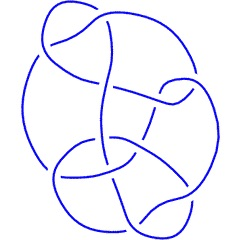
\includegraphics[width=5cm]{Images/Conway knot.jpeg}}}
    \qquad
    \subfloat[\centering Unknot]{{
\includegraphics[width=5cm]{Images/unknot.jpeg}}}%
    \caption{The Conway knot (a), an 11 crossing knot, shares the same Alexander-Conway polynomial as the unknot (b).}%
    \label{knot_comp}%
\end{figure}

This is a classification problem; finding a way to distinguish between each \emph{class} of knots (unknot, Conway knot...) given specific \emph{features} (Alexander-Conway polynomial, DT code, XYZ position...).

Machine learning methods make use of algorithmic frameworks to probabilistically determine a mapping function (f) given a set of input features ($\vec{X}$) and their corresponding output (y). Through this, machine learning methods provide solutions to classification problems, and so we seek to apply these methods to investigate the classification of knots.

Building on prior work by Sleiman et.\ al.\ \cite{sleiman2022geometric} in which it was successfully found that the segment-to-segment writhe of a knot resulted in near perfect ($\approx99\%$) classification \footnote{up to 10 crossings}, we ask ourselves if this result is consistent when trained in an unsupervised environment, one in which the machine learning model is not given the labels of the corresponding data. Ultimately we want to find if the machine learning model is able to identify its own labels and classify its data unprompted. As a result, the model would be able to distinguish between knots, generate a latent space with discrete mapping of the different types of knots and additionally, generate new knots based on it's learned parameters (specifically knots on which the model was not trained). 
In doing so, we learn more about the underlying mathematical mechanism by which segment-to-segment writhe leads to classification of knots and seek to understand the repercussions of this from a physics point of view.

This report will tackle how this was completed and the results found. 
However first, a background on knot theory, machine learning and generative machine learning will be presented to give the reader sufficient context for the discussions that follow.


\hl{Road map:}

    1. Fundamentals:
   - ML Fundamentals: Basics of machine learning. 
   Supervised and unsupervised learning, neural networks, and the fundamentals of how models learn from data.

   - Generative Models: Generative Adversarial Networks (GANs) and Variational Autoencoders (VAEs).

   - Knot Theory Basics: Review the fundamental concepts of knot theory. Understand the different types of knots, their properties, and how they can be represented.

    2. Literature Review:
   - Relevant Research Papers: Machine learning and knot theory. 
   Importantly -> note: state-of-the-art techniques, challenges, and gaps in the existing literature.

   - Explore Applications: Investigate how generative machine learning has been applied in other mathematical and physical domains -> any insights or methodologies that can be adapted to knot theory?

    3. Specific Problem or Question:
   - Define Scope: Narrow down focus within the intersection of generative machine learning and knot theory.

   - Identify Challenges: Challenges that arise in applying generative machine learning to knot theory. This could include issues related to data representation, model complexity, or interpretability.

    4. Data Collection and Preparation:
   - Data Availability: Use of existing dataset.

   - Data Preprocessing: Clean and preprocess data to ensure it's suitable for training machine learning models. This may involve normalizing, scaling, or transforming your knot data (should already be done).

    5. Experimentation and Model Development:
   - Pytorch.

   - Model Architecture: Design generative model architecture.

   - Training and Evaluation: Train model using appropriate algorithms and evaluate performance. Iterate on model based on the results.

    6. Interpretation and Analysis:
   - Interpret Results: Analyze results of experiments. Evaluate generative models ability to produce \emph{meaningful} instances of knots.

   - Implications: Implications of findings on knot theory. How can generative machine learning contribute to the understanding or discovery of new aspects of knots.

   7. Conclusions:
   - Future Work: Directions for future research in the intersection of generative machine learning and knot theory.



\section{Background}

% \begin{it}
% The background section is where you set out, in a self-contained way, the key concepts that it is essential for the reader to understand in order to make sense of the results. This would also be an appropriate place to discuss other attempts in the literature to solve the problem you are faced with, and critique the successes and limitations of these. By the end of this section, the reader should have some understanding of what would count as a successful outcome from the project.
% \end{it}

% \LaTeX\ is the standard software for typesetting technical documents (like research papers and project reports) in the mathematical and physical sciences (although it is increasingly used in other fields as well). Unlike other document preparation software that you might be familiar with, like Microsoft Word, you do not write directly onto the page. Instead, you write your text a \emph{source file} that contains regular text (like this) as well as a set of commands that allow other material---notably figures and equations---to be inserted.  These commands are introduced with a backslash character; arguments to these commands are placed inside pairs of curly brackets.

% For example, to emphasise text, you use the command \verb|\emph{emphasised text goes here}| which renders as \emph{emphasised text goes here}. Throughout this document, we will use \verb|this font| to denote \LaTeX\ source code (or commands to be entered at the command line, see below).

% The process of converting your \LaTeX\ source to a readable document is referred to as \emph{typesetting} or \emph{compiling} your document (the latter in analogy to compiling human-readable source code in a language like C or C++ to a code that can be executed by the computer). How this is done depends on the environment you are writing your source code in:
% \begin{itemize}
% \item The classical approach is to edit your source in a text editor, like \verb|emacs| or \verb|vi| (if you are super old-school), and run the typesetting engine from the (Linux, MacOS or Windows) command line. Usually the program that you will want to run is called \verb|pdflatex|, which can incorporate figures in PDF, PNG and JPEG format, and outputs a PDF document. If your sourcefile is called \verb|darkmattereport.tex| it is run like this (\verb|$| denotes a shell command prompt):

% \begin{verbatim}
% $ pdflatex darkmatterreport
% \end{verbatim}

% This will generate typically a lot of output, and leave a file called \verb|darkmatterreport.pdf| in the same folder (directory) as the source file. You can look at this in a PDF viewer, like Adobe Reader. Modern PDF viewers should be able to detect when the document has been updated, and refresh automatically.

% This approach will work in the CPLab, and most likely also on your own computer, whether Linux, MacOS or Windows based.
% %
% \item The more modern approach is to use an dedicated \LaTeX\ editor, which will usually have buttons or keyboard commands that compile and display the output for you. The standard \LaTeX\ distribution for macOS users is \href{https://tug.org/mactex/}{Mac\TeX} which comes with an app called \TeX Shop (if you install the GUI apps alongside): this is a very user-friendly editor. The standard distribution for Windows users is \href{https://www.tug.org/texlive/}{\TeX\ live} and comes with the \TeX works editor. \TeX works also runs on macOS and Linux.
% %
% \item An increasingly popular alternative to a desktop app is to use a web-based \LaTeX\ editing service, like \href{https://www.overleaf.com}{Overleaf} or \href{https://www.sharelatex.com}{Share\LaTeX}. One advantage of these is that you do not have to install \LaTeX\ on your own machine (which has quite a hefty footprint), and you will get the same view of the document from different machines (e.g., Linux hosts in the CPLab, Windows-based machines in the library, your own laptop etc). The downside is that you do need an internet connection, and compilation can be slow.
% \end{itemize}

% Fortunately, \LaTeX\ is very mature and quite standardised, so you should find your documents can be ported easily between different environments if required. The main issue is whether any packages you use are installed, but unless you use extremely obscure packages, this is unlikely to be an issue.

% In the next section we outline some of the key features of \LaTeX\ and most commonly-used commands. However, \LaTeX\ is a vast, highly configurable system that we cannot describe exhaustively in such a short document. Instead we refer you to the following places for more information:
% \begin{itemize}
% \item The \href{https://www.wiki.ed.ac.uk/x/7y6UCw}{source code} to this document, which will allow you to see how it was created!
% %
% \item \href{https://www2.ph.ed.ac.uk/~wjh/tex/ilw/slides-beamer.pdf}{Will Hossack's Short Introduction to \LaTeX}.
% %
% \item \href{https://www.latex-tutorial.com/tutorials/}{An online step-by-step guide to \LaTeX}.
% %
% \item The book \textit{A Guide to \LaTeX} by Kopka and Doly \cite{Kopka2003}.
% %
% \item The \href{https://tex.stackexchange.com}{\TeX-\LaTeX\ stack exchange}, a board where questions and answers on aspects of \LaTeX\ (and a lower-level system called \TeX\ that it is built on) are posted.
% %
% \item A search engine known as \href{https://www.google.com/}{Google}, which you may have heard of.
% \end{itemize}

\subsection{Knot theory}
\subsubsection{Knot classification}

\subsection{Machine learning}
\subsubsection{The classification problem}
\subsubsection{Neural networks}

\subsection{Generative Machine learning}
\subsubsection{The Autoencoder}
\subsubsection{GAN's and VAE's}
\hl{Examples}

\section{Methods}

% \begin{it}
% The methods section is a description of what you did. In an experimental project, this would comprise a description of your apparatus and the protocol you followed to obtain the measurements. In a simulation project, this would be a description of the simulation method. In a more mathematical project, there may not be any ``methods'' as such: for example, the main ideas and techniques you are developing might fall more naturally into the background / literature review section, and the application of these might be regarded as results. In this case you might decide to skip an explicit ``methods'' section.
% \end{it}

% \subsection{Structure of the document}

% The source file minimally contains:
% \begin{verbatim}
% \documentclass[12pt]{article}
% \usepackage{mphysproject}

% \begin{document}

% \end{document}
% \end{verbatim}

% If you are enrolled on the MPhys with a Year Abroad degree programme, you will be doing a shortened version of the project, for which a shorter project report is expected. If this applies to you replace the \verb|usepackage| line above with
% \begin{verbatim}
% \usepackage[yearabroad]{mphysproject}
% \end{verbatim}


% The document text goes in between the \verb|\begin{document}| and \verb|\end{document}| pair. The \verb|mphysproject| package is non-standard and has to be placed in the same folder as your source document. This package comprises the files \verb|mphysproject.sty| and \verb|PandA_black.pdf|, the latter of which is the School of Physics and Astronomy logo that appears on the title page.

% Paragraphs of text are separated by blank lines in the source document: line breaks are ignored. \LaTeX\ automatically adds an extra bit of space after full stops, which it interprets as marking the end of a sentence. Sometimes a full stop is not a full stop, e.g.\ following an abbreviation (like e.g.). You can set a normal size space by preceding it with a backslash: \verb|i.e.\ like this|.

% Sections are introduced with the command
% \begin{verbatim}
% \section{Section title}
% \end{verbatim}
% and within sections, you can have \verb|\subsection{...}| or \verb|\subsubsection{...}| if required, though you probably don't need to go any deeper than the \verb|\subsection{...}| level. 

% The \verb|mphysproject| style file redefines a few standard commands, and adds some non-standard commands to help you structure and format your document according to the rules set out in the Course Information Booklet.

% \subsubsection{Title page}

% At the start of the document (just after \verb|\begin{document}|) you should define the contents of the title page with the following commands:
% \begin{verbatim}
% \title{Title of your project} 
% \author{Your name}
% \supervisor{Your supervisor's name}
% \date{Submission date}

% \begin{abstract}
% Abstract text
% \end{abstract}

% \maketitle
% \end{verbatim}

% Repeat the \verb|supervisor| line if you have multiple supervisors, with one supervisor per \verb|\supervisor| command. The \verb|\maketitle| line at the end is essential, as without it the title page won't appear!

% \subsubsection{Personal statement}

% Before your personal statement, insert the line
% \begin{verbatim}
% \personalstatement
% \end{verbatim}
% This provides an appropriate heading.

% \subsubsection{Main text and automatic length check}

% After the personal statement and any acknowledgements, and before beginning the introduction you \emph{must} include the command
% \begin{verbatim}
% \maintext
% \end{verbatim}

% This does three things:
% \begin{enumerate}
% \item It inserts a Table of Contents.
% \item Switches the page numbering from Roman numerals to Arabic numbers.
% \item It starts counting pages for the automatic length check.
% \end{enumerate}
% If you don't include this command, three bad things happen. First, you don't get told if your report is over length. Second, Roman numerals start to look silly when the numbers get too big.  Third, it makes it hard to do the length check manually.  The pages numbered $1$, $2$, $3$, \ldots are those that are significant in terms of determining the page count for the project. These appear only if \verb|\maintext| is placed before the introduction.

% Note that \verb|\maintext| does \emph{not} start a section called `Introduction': this you must insert yourself with
% \begin{verbatim}
% \section{Introduction}
% \end{verbatim}

% The automatic length check ends either with the end of the document, or the start of the appendices, whichever comes first. If the page limit is exceeded, a warning appears in the document at this point. (It also appears in the output from \LaTeX\ that appears on the command line, although this is easy to miss).

% \subsubsection{Appendices}

% If you are including (non-assessed) appendices in your document, insert the line
% \begin{verbatim}
% \appendix
% \end{verbatim}
% at the end of your conclusion, and before the first appendix. Each appendix should be introduced with its own \verb|\section{...}| command.

% A note will be inserted into the document at the beginning of your appendices to remind you and the markers that the contents of the appendices are disregarded for the purposes of assessment.


% \subsection{Special characters and emphasis}

% \LaTeX\ was invented at a time when only a small number of characters could be reliably entered from a keyboard: therefore `special' characters have to be entered manually (i.e., using commands). These include:
% \begin{itemize}
% \item \emph{open and close quotes} --- Open quotes are entered as backticks and close quotes as apostrophes, that is \verb|`| gives ` and \verb|'| gives '. To get double quotes, double up the characters: \verb|``like this''| gives ``like this''.
% \item \emph{dashes and hyphens} --- \LaTeX\ provides three lengths of hyphens/dashes. Typing a single \verb|-| gives you a hyphen, used for hyphenating words (e.g., first-order phase transition). Typing a double \verb|--| gives you a short dash, used for ranges of numbers (e.g., 1--99). Typing a triple \verb|---| gives you a long dash---often used to introduce subclauses.
% \item \emph{accented characters} --- \LaTeX\ gives access to a large number of accents, which may be useful if you want to refer to copiously-\"{u}ml\"{a}\"{u}t\"{e}d heavy-metal bands, for example. Do a Google search on `latex accents' to see how to get them.
% \end{itemize}

% The two most common types of emphasis you might wish to employ are \textit{italics} and \textbf{bold face}, which were set with \verb|\textit{italics} and \textbf{bold face}|. Purists prefer the \verb|\emph{...}| command, as this expresses the notion that it is emphasis that you want, rather than bold or italics specifically. \LaTeX\ will choose an appropriate emphasis, which is usually italics.

% \subsection{Equations}

% The reason that \LaTeX\ has established itself as \emph{the} typesetting system for physicists and mathematicians is that it allows complex equations to be included in your document with ease. Whole books have been written on this subject. However, about $95\%$ of your needs are provided for by the following tips.

% \begin{itemize}
% \item There are two (main) ways to include equations. The first is to include them inline. For example, Newton's second law can be written as $F = ma$, which is typeset as \verb|$F = ma$|. A single dollar sign opens and closes an inline equation. The second type of equation is a displayed equation. For example, the partition function of the quantum mechanical harmonic oscillator is
% \begin{equation}
% \label{Z1}
% Z(1) = \frac{{\rm e}^{-\frac{\hbar\omega}{2kT}}}{1 - {\rm e}^{-\frac{\hbar\omega}{kT}}} \;.
% \end{equation}
% In the source document, this equation is written as
% \begin{verbatim}
% \begin{equation}
% Z(1) = \frac{
%   {\rm e}^{-\frac{\hbar\omega}{2kT}}}
% }{
%   1 - {\rm e}^{-\frac{\hbar\omega}{kT}}}
% } \;.
% \end{equation}
% \end{verbatim}
% There are many mathematical symbols you can include: tables of these symbols can be found by doing a Google search on `latex math symbols'. Sometimes you need to include additional packages (like \texttt{amsmath} or \texttt{amssymb}) to use more exotic symbols.

% Try and use the right symbols where you can. For example, a common error is to use greater-than and less-than signs instead of angle brackets (\verb|\langle| and \verb|\rangle|). Good: $\langle E \rangle$ and $|\psi\rangle$. Bad: $< E >$ and $|\psi>$.
% \item If you have brackets around sums, integrals, fractions or other large objects, use \verb|\left| and \verb|\right| so that they are automatically made large enough to enclose their contents. Compare for example
% \begin{equation}
% \left( \sum_{k=0}^{\infty} z^k \right) \;,
% \end{equation}
% typeset as \verb|\left( \sum_{k=0}^{\infty} z^k \right)|, as opposed to
% \begin{equation}
% ( \sum_{k=0}^{\infty} z^k ) \;,
% \end{equation}
% which does not use \verb|\left| or \verb|\right|.
% \item The mysterious error `You cannot use \verb|\eqno| in math mode' means that you have forgotten a \verb|\right| that is needed to match a \verb|\left|.
% \item Always use the \verb|\begin{equation}| \ldots \verb|\end{equation}| environment for displayed equations, rather than one of the other options available to you. This makes sure that an equation number appears. Even though you may not refer to a particular equation, someone else might want to!
% \item Equations should be punctuated as normal text. So if a displayed equation ends a sentence, place a full stop at the end of it. It helps to insert a little bit of spacing, using \verb|\;| before this punctuation.
% \item It is tempting in the source to insert blank lines before and after equations for readability. Do not do this, as this starts a new paragraph (inserting extra space) each time. Only put a blank line if the paragraph has genuinely ended.
% \item Some people insist that exponential ${\rm e}$ and total derivatives ${\rm d}$ should be set in roman font using \verb|{\rm e}| and \verb|{\rm d}| whilst others find this overly fussy.
% \item However, everyone agrees that you should set things like $\sin x$ and $\cos x$ using \verb|\sin x| and \verb|\cos x| and not as \verb|sin x| and \verb|cos x|, as the latter come out as $sin x$ and $cos x$: that is, these read as the variable $s$ times $i$ times $n$ times $x$ and as $c$ times $o$ times $s$ times $x$, and not what you actually want.
% \end{itemize}

% \subsection{Figures and tables}

% The \verb|mphysproject| package includes a set of commands (inherited from the \verb|graphicx| package) that allow you to include figures in PDF, PNG and JPEG formats directly into the report. See Figure~\ref{fig:cmbr} for an example, where the original image lies in a file called \verb|Cmbr.pdf|.

% A figure is a special kind of object called a \emph{float} that \LaTeX\ positions separately to the text, usually somewhere near the point at which it is embedded in the source code. The typical sequence of commands is
% \begin{verbatim}
% \begin{figure}[htb]                
% \begin{center}
% \includegraphics[width=10cm]{filename}
% \end{center}
% \caption{\label{reference_label} Caption goes here.}
% \end{figure}
% \end{verbatim}

% The \verb|\begin{figure}| \ldots \verb|\end{figure}| pair encloses the floating material that can be reposition. The referenced external file should lie in the same folder as the \LaTeX\ source document. You can leave the extension (\verb|.pdf| etc) off the filename, and \LaTeX\ should still find it. See Section~\ref{sec:ref} below for more information about the reference label.

% \begin{figure}[htb]                % h = here; t = top (of page); b = bottom (of page)
% \begin{center}
% \includegraphics[width=10cm]{Cmbr} % Vary the value in the width=XX setting to resize the figure if need be.
% \end{center}
% \caption{\label{fig:cmbr} The cosmic microwave background radiation spectrum, adapted from the Wikipedia page \cite{Cmbr}. The line is Planck's formula, and the crosses are observational data (errors are smaller than symbol size). Note the close correspondence between the two.}
% \end{figure}

% When starting out with \LaTeX\ it is natural to attempt to wrest some control over the placement of figures. Let me save you several months of your life at the outset, and recommend you just let \LaTeX\ get on with it. Your main control over the display of the figure lies in where the \verb|\begin{figure}| \ldots \verb|\end{figure}| block appears in the text. If the figure comes too soon, move it later; if it comes too late, move it earlier. The three characters \verb|htb| comprise a set of polite requests as to where you want the figure to go: \verb|h| means `here', \verb|t| means `at the top of a page' and \verb|b| means `at the bottom of a page'. We say \emph{a} page (not \emph{this} page) advisedly. You can add an exclamation mark \verb|!| to make a less polite request; \LaTeX\ may nevertheless rudely ignore it. You can adjust the size of the figure by changing \verb|width=10cm| to something else. You can put two figures side by side above the same caption by repeating the \verb|\includegraphics| line (and adjusting the filename appropriately).

% A similar construction, enclosed by a \verb|\begin{table}| \ldots \verb|\end{table}| pair is available for the inclusion of tables. Again you can add the \verb|htb| request to exert some influence over where it appears. See Table~\ref{tab:atable} for an example. You are referred to the source, and in particular \cite{Kopka2003} who are unusually enthusiastic about tables, for information about how the tabulated content is marked up in \LaTeX.

% \begin{table}[htb]
% \begin{center}
% \begin{tabular}{l|l|l} % This specifies three left-justified columns separated by vertical lines. Change l to r or c to get right-justified or centred columns; add more columns if you need them
% Particle type & Spin & Multiple occupancy allowed \\\hline\hline % Columns are separated by &, rows by \\
% Bosons & Integer & Yes \\
% Fermions & Half-integer & No \\\hline % An \hline after a row separator \\ puts a horizontal line after the row
% \end{tabular}
% \end{center}
% \caption{\label{tab:atable} Summary of the key properties of fermions and bosons.}
% \end{table}


% \subsection{Cross-referencing within the document}
% \label{sec:ref}

% The second most useful feature offered by \LaTeX\ (after its unparalleled equation typesetting abilities) is being able to label numbered items in the text, and refer to them later by that label. This is useful because if you reorganise the text (e.g., add extra figures) which causes items to be renumbered, all the cross-references automatically update.

% To create a label, insert \verb|\label{reference_label}| in the text. To refer to the labelled item, insert \verb|\ref{reference_label}| in the text. For example, this current subsection, numbered \ref{sec:ref}, is labelled \verb|sec:ref|. There is an apparently unwritten but widely-used convention of `namespacing' the labels so that section labels all begin with \verb|sec:|, figures with \verb|fig:| etc, but you don't have to do this.

% \LaTeX\ is pretty smart about knowing \emph{what} is being labelled. If you place the label among the regular text, it will refer to the current section. If you place it inside a \verb|\begin{equation}| \ldots \verb|\end{equation}| pair, it will label the equation. It seems figures and tables are mostly reliably labelled if you include the \verb|\label| inside the caption. Alas \LaTeX\ is less smart about referring to the label; for example, if you want to refer to an equation, you have to manually type the brackets around the equation number: \verb|(\ref{Z1})| gives (\ref{Z1}); likewise you will need to include the word `Figure' when referring to Figure~\ref{fig:cmbr}: \verb|Figure~\ref{fig:cmbr}|. (Note the \verb|~| here stops the word Figure and the figure number appearing on different lines of text, which some people find unappealing).

% It is worth having a little understanding of how the cross-referencing system works under the hood. As your source file is compiled, \LaTeX\ creates a file with the extension \verb|.aux| that records what each label refers to. This auxiliary file is read in when compilation starts. What this means is that when you \emph{first} compile the document, it won't actually know what a label refers to, as this information isn't in the auxiliary file yet. As this point, references appear as question marks (?). So you have to compile it again to get the references to appear correctly. Very occasionally, you might need to compile a third time, as sometimes the formatting of the document can change due to the correct label text being inserted. This goes particularly for the table of contents, as page numbers might change with the formatting. Before submitting your report, it is usually a good idea to make sure you have run \LaTeX\ multiple times, and look out very carefully for warnings about missing references in the log that it produces.

% \subsection{Referencing external sources}

% A similar command is provided for citing papers, textbooks, webpages etc. Each item in the list of references has a label (also called a key), and a citation is inserted in the text with the command \verb|\cite{label}|. For example, \verb|\cite{Kopka2003}| gives the citation \cite{Kopka2003}. If you want to cite multiple works at the same point in the text, do it like this: \verb|\cite{Kopka2003,Cmbr,Askin1986}| which appears as \cite{Kopka2003,Cmbr,Ashkin1986}. Treat the citation as a word in the text: that is, it should be preceded by a space, and followed either by a space or a piece of punctuation.

% We defer a discussion of how the reference list is constructed, and its items labelled, to the References section below (Section~\ref{sec:refs}).

Having now laid out the fundamentals, we investigate the implementation of generative machine learning techniques to explore the classification of knots using segment-to-segment writhe.

\hl{Considerations for designing the model architecture}:

    1. Data
   - Data Representation: How is the knot data represented. Design input layer to accommodate this representation.

   - Data Complexity: Consider complexity of knot data. Some knots might have simple structures, while others can be highly intricate. Model architecture should be variable to capture this complexity.

    2. Generative Model:
   - GAN -> generating realistic data.
   - VAE -> learning a probabilistic distribution of the data.

   - Hybrid Model -> Hybrid approach to combine both VAE and GAN (will need to research).

    3. Encoder and Decoder Architecture:
   - Encoder: (VAE or hybrid) -> encoder maps input knot data to a latent space representation. 
   Convolutional layers work well for \emph{spatial} features.

   - Decoder: decoder maps latent space back to the original data space. 
   Important! -> output layer matches input.

    4. Loss Function:
   - Adversarial Loss: (GAN). Coupled with a discriminator that distinguishes between real and generated knots.

   - Reconstruction Loss: (VAE). Helps model learn underlying distribution of data.

    5. Considerations for Knot Theory:
   - Topological Features: Ensure that model architecture can capture and generate features.

   - Invariant Representations: Make model invariant to certain transformations that don't change the underlying knot structure. eg, chirality + mirroring.

    6. Hyperparameter Tuning:
   - Learning Rate (test).

   - Batch Size (test).

   - Architecture Depth and Width: (test) depth and width of nn layers.

    7. Regularization and Normalization:
   - Dropout layers: prevent overfitting.

   - Batch Normalization: Normalize inputs to each layer -> faster convergence and better generalization.

    8. Validation and Testing:
   - Validation Set: check OG code.

   - Early Stopping: check OG.

    9. Visualization:
   - Visualization: PCA and t-SNE visualize latent space and see how model is separating different types of knots.



\section{Results and Discussion}

% \begin{it}
% In many cases, the results will take the form of graphs. If you have many results, you do not need to include them all: select the ones that are most significant. This goes also if your results take the form of a calculation: it is not necessary to give all intermediate steps, but enough detail should be included to allow a person competent in the field to follow the general route taken and, if necessary, reconstruct missing steps. Try to avoid unnecessary repetition.
% \end{it}

% In the previous section, we covered the mechanics of including figures and tables into your report. We now turn to some considerations of good practice regarding your results and discussion of them. Perhaps the most obvious one of these is that figures should be displayed at a size that all text and relevant features is legible. Perhaps the next most obvious is that you should refer to every figure (and table) in the text. The usual procedure is to specify first the relevant conditions under which the results were obtained (e.g., simulation parameters, choice of experimental protocol etc), and then refer to the figure. You should make clear what is learnt by looking at the figure: that is, what is plotted as a function of what, and what the physically significant features are (e.g., is it the location of a peak? the difference between two curves? the behaviour at large or small values along one of the axes?). The caption should generally do these things to, but in a more terse manner. For example, in the case of Figure~\ref{fig:cmbr}, the key point is that the theoretical prediction (given by Planck's formula) and the observation data show an extremely close correspondence.

% Try to avoid including many similar looking figures. Often it is better to show one representative figure, and explain that other conditions yield similar results; or to plot a single quantity as a function of the relevant control parameter to show what does (or doesn't change). Remember to discuss sources of error.

% In more mathematical projects, the results may take the form of (a perhaps fairly extended calculation). Again, you do not need to include all the steps; and if you perform several calculations of the same basic type, then it may be appropriate to use the first calculation to set out the method in detail, and then skip parts of later calculations when they are essentially the same as what has already been presented.

\section{Conclusion}

% \begin{it}
% In the conclusion you should bring together your main findings, and explain what we have learnt from them collectively. You should refer back to the broader research area and outstanding questions alluded to in your introduction, and make clear what progress has been made towards understanding them as a result of the project. Suggestions for further work should also go here.
% \end{it}

% In this template document, we have provided a very brief introduction to creating a project report using \LaTeX, with particular emphasis on the special features of the \verb|mphysproject| package that simplify the process of creating a report that is compatible with the requirements for the MPhys Project course. As has been stated on a number of occasions, we are only able to scratch the surface of what is possible, although it should cover the vast majority of your needs. You are reminded that this document includes only a precis of the guidance that is available on the MPhys Wiki, links to which were provided in the Introduction.



\appendix

\begin{it}
(NB:  the above message is automatically inserted by the \verb|\appendix| command and you should not attempt to remove it).
\end{it}

% \section{Using Bib\TeX\ to manage your references}
% \label{sec:bibtex}

% As noted in Section~\ref{sec:refs} in the main text, it is quite a laborious task to construct a bibliography manually, and we recommend that instead you keep a separate database of references in Bib\TeX\ format. This database is a text file with its own markup conventions; again there are apps that will allow you to create and manage it in a more user friendly way, for example, \href{http://www.jabref.org}{\texttt{Jabref}} works on Linux, macOS and Windows, and the Mac\TeX\ distribution comes with an app called \texttt{BibDesk} that is very easy to use.

% Like \LaTeX\, Bib\TeX\ is a very complex application capable of many things. We will again only scratch the surface here, and again this will likely be sufficient for the needs of an MPhys project. We refer you to the \href{https://en.wikipedia.org/wiki/BibTeX}{Bib\TeX\ Wikipedia page} for more details and some links.

% The references themselves go into a file with a name ending in \verb|.bib|, for example, \verb|mphys-refs.bib|.  The Bib\TeX\ file for this document contains just three references, and looks like this
% \begin{verbatim}
% @article{Ashkin1986,
%    Author = {A Ashkin and J M Dziedzic and J E Bjorkholm and S Chu},
%    Journal = {Optics Letters},
%    Pages = {288--290},
%    Title = {Observation of a single beam gradient 
%             force optical trap for dielectric particles},
%    Volume = 11,
%    Year = 1986}

% @book{Kopka2003,
%    Address = {Boston},
%    Author = {H Kopka and F W Daly},
%    Edition = {4th},
%    Publisher = {Addison-Wesley},
%    Title = {Guide to \LaTeX},
%    Year = 2003}

% @misc{Cmbr,
%    Note = {\url{http://en.wikipedia.org/wiki/Cosmic_microwave_background}. 
%            Accessed 1st Jan 2017},
%    Title = {Cosmic microwave background, {Wikipedia}}}
% \end{verbatim}

% This example should be sufficient for you to be able to reverse-engineer most of the BiB\TeX\ file format. Entries are of the form \verb|@doctype{label, key-value-pairs}|. The two most common \verb|doctype|s are \verb|book| or \verb|article| (the latter being an article published in a research journal). The full set of types depends on the style file you use (see below): other types that are usually supported are \verb|mastersthesis|, \verb|phdthesis| and \verb|proceedings| for Masters and PhD thesis and conference proceedings, respectively. The \verb|misc| document type is a general purpose type that can be used when nothing else fits. Traditional Bib\TeX\ style files are pre-internet, and so are hazy on the notion of URLs for example. The above is one strategy you can use to reference web pages.

% The \verb|label| that appears after the \verb|doctype| is the one that you will put inside the \verb|\cite| commands in your \LaTeX\ source. The \verb|key-value-pairs| are of the form \verb|key={value}|, and define things like the authors, the book title and so on. The braces around the \verb|value| are optional if the value is a number. Each key-value pair is separated by a comma. Two things to note are that each author in a list of authors must be separated with the word \verb|and|. Also, Bib\TeX\ will attempt to make things like the case of different entries consistent, sometimes by downcasing capitalised words. You can stop this happening by placing such words in curly brackets, as with \verb|{Wikipedia}| in the above example. You also need to use curly brackets if an author has a surname that comprises two separate words (i.e., without a hypen), as for example in the case of \verb|John {Maynard Smith}|, whose surname was Maynard Smith, and not Smith. Bib\TeX\ will think that Maynard is a middle name if you don't use curly brackets.

% To tell \LaTeX\ to use an external bibliography file, you need to insert two commands into your source. The first tells Bib\TeX\ the style file to use. This determines which document types and key-value pairs are allowed, and also how these are converted into a common format in your list of references. This command is
% \begin{verbatim}
% \bibliographystyle{unsrt}                      
% \end{verbatim}
% where \verb|unsrt| is one of the basic style sheets, and lists your references in the order that they are cited (which is the usual convention in physics). This command can appear anywhere in the \LaTeX\ document, e.g., in the preamble (the part before \verb|\begin{document}|) or at the point where the bibliography appears in the report.

% The second command actually inserts the source code for your bibliography into the document, and therefore \emph{must} appear at the point where you want it. This command is
% \begin{verbatim}
% \bibliography{mphys-refs}
% \end{verbatim}
% where the argument should have the same name as your Bib\TeX\ database file (but with the \verb|.bib| extension left off).

% To get the bibliography to actually appear, and for all the citations to refer to the correct item, you have to run \LaTeX\ and Bib\TeX\ a number of times. Assuming you are working from the command line on in the CPLab you would do, and your \LaTeX\ file is called \verb|project-report.tex|, you would do:
% \begin{itemize}
% \item \verb|pdflatex project-report| --- on the first pass, the label in each \verb|\cite| command will be output into the auxiliary (\verb|.aux| file, see Section~\ref{sec:ref}) files, as will information about the style file and database(s) that Bib\TeX\ needs to refer to.
% \item \verb|bibtex project-report| --- Bib\TeX\ now reads in the \verb|.aux| file, locates the database of references, and then goes through the items you have cited to construct the \LaTeX\ source for the bibliography in the format specified by the style file. This source code is inserted into a file with extension \verb|.bbl|. (You can look at this if you want).
% \item \verb|pdflatex project-report| --- on the second pass, \LaTeX\ reads in the \verb|.bbl| file at the appropriate point. As with cross-references, \LaTeX\ does not yet know which label has which number, so at this stage all citations will appear as `?' in the text. However, this information is written into the \verb|.aux| file on this second pass.
% \item \verb|pdflatex project-report| --- on the third pass, the information \LaTeX\ needs to resolve the references (i.e., insert numbers at the point where references are cited) is now in the \verb|.aux| file, and these can be inserted.
% \end{itemize}
% Exceptionally, one further compilation might be required if the insertion of numbers into the citations causes the page layout to change, and page references become outdates. However, this is very rare. Friendly front-end apps to \LaTeX\ and Bib\TeX\ may provide commands that perform the multiple runs for you automatically.

% You only need to re-run \verb|bibtex| if you cite new references, or if you change the order that references are cited in (as in this case a new bibliography will need to be constructed). Consequently, after most edits to your source file, a single run through \LaTeX\ should be sufficient. However, before submitting your report, it is worth going through the full \LaTeX\-Bib\TeX\ cycle as described above, with additional runs of \LaTeX\ until any warnings about undefined references or citations go away. (It may be that you have misspelt a reference label, or omitted a reference from the \verb|.bib| file, so you should check the \LaTeX\ log carefully to fix such things).


\newpage
\printbibliography

\end{document}